
\documentclass{beamer}
% \usetheme[secheader]{boxes}
\usecolortheme{default2}
% \usecolortheme{default}

\usepackage{lmodern}
%\usepackage[inline]{enumitem}   
% \usepackage[latin1]{inputenc}
% \usepackage{xcolor}
% \usepackage{fontenc}
\usepackage{tcolorbox}
\usepackage{latexsym}
% \usepackage{multirow}
\usepackage{amsmath,amsthm,amssymb,color}
\usepackage{array}
\usepackage{fancybox}			% For box
\usepackage{enumerate}

%---------------------------------------------------------------------------
% for \coloneqq
\usepackage{mathtools}

%---------------------------- for tikz -------------------------------------
\usepackage{tikz,tabularx}
\usetikzlibrary{decorations.pathreplacing}
\tikzstyle{every picture}+=[remember picture]
\usetikzlibrary{shapes,arrows,shadows}	
\usepgflibrary{patterns}
\usetikzlibrary{patterns}
\usetikzlibrary{shapes.geometric}
\usetikzlibrary{arrows}
\usetikzlibrary{decorations.pathreplacing}
\tikzstyle{every picture}+=[remember picture]

\setbeamertemplate{blocks}[rounded][shadow=true]

\usetikzlibrary{positioning}

\usepackage{multicol}
\setlength{\columnsep}{1cm}

\usepackage{pgfplots}
\pgfplotsset{major grid style={densely dotted,black!70}}
\pgfplotsset{compat=1.9}

%--------------------- give numbers to frames  -----------------------------
\setbeamertemplate{footline}[frame number]

%------- to remove navigation symbols at right bottom corners --------------
\setbeamertemplate{navigation symbols}{}

%-------------------------------------------
% For curved arrows
% \draw [->,red, thick] (0,0) -- (1,1) --(4,0)--(5,0) --(5,1)--(4,1);      
% \draw[->] (0,0) .. controls (1,1) .. (4,0) .. controls (5,0) and (5,1) .. (4,1);

%--------------------------- new definition shortcuts ----------------------
\def \mp {\pause}
\def \mp {}

%=================================================================

\newcommand{\ft}[1]{\frametitle{#1}}
\newcommand{\tcr}[1]{\textcolor{red}{#1}}
\newcommand{\tcb}[1]{\textcolor{blue}{#1}}
%\newcommand{\st}{\ensuremath \mathit{x}}
\newcommand{\mc}[1]{\mathcal{#1}}
\newcommand{\pr}{\mathbb{P}}
\newcommand{\sa}{\mathit{\sigma-}algebra}
\newcommand{\ninf}{n \rightarrow \infty}
\newcommand{\ninfu}{\limits_{n \rightarrow \infty}}
\newtheorem{defi}{Definition}
\newcommand{\borel}{\mathcal{B}(\mathbb{R})}
% \begin{frame}
%  \begin{figure}[t]
%   
%   \begin{tikzpicture}
%   
%   \end{tikzpicture}
% 
%   \end{figure}
% \end{frame}



\begin{document}

\begin{frame}
 
\begin{figure}[t]

    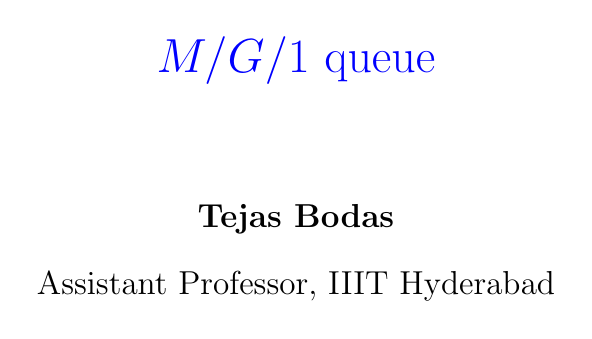
\begin{tikzpicture}


        \node [above] at (0,0.5) {\LARGE \textcolor{blue}{$M/G/1$ queue}};


        \node [above] at (0,-1.4) {\large \textbf{Tejas Bodas}};	  

        \node [above] at (0,-2.25) {\large Assistant Professor, IIIT Hyderabad};


%        \node [above] at (0,-3.3-0.12) {\footnotesize PhD: IIT Bombay};	  

 %       \node [above] at (0,-3.25-0.7-0.12) {\footnotesize Post-doc:~~TIFR, LAAS-CNRS (France), University of Antwerp (Belgium), IISc};

  %      \node [above] at (0,-3.25-0.7-0.6-0.22) {\small Area of research : performance modelling, resource allocation};
        
   %     \node [above] at (0.4,-3.35-0.7-0.6-0.52) {\small queueing theory, game theory};

%         \node [above] at (0.4,-3.75-1-0.6-0.52) { (Stochastic processes)};
    \end{tikzpicture}

\end{figure}
 
\end{frame}


\begin{frame}
 \ft{Age and Residual life of a Renewal process}\begin{figure}
\includegraphics[width=7cm]{renewal}
\centering
\end{figure}
\begin{itemize}\setlength\itemsep{.8em}
 \item Let $A(t)$ and $R(t)$ denote the age and the residual life of the renewal process at time $t$.
 \mp\item Assume you arrive at a Metro station at time $t$.
 \mp \item $A(t)$ is the time since the last metro departed.
\mp \item $R(t)$ is the time till the next Metro arrives.

\mp \item Assume that you arrive uniformly at random to the Metro. 
\mp \item What is your average waiting time $\bar{R}$ ? $\bar{R} = E[X]/2$?
 \end{itemize}


\end{frame}


\begin{frame}
 \ft{Hitchhiker's Paradox!}
 \begin{figure}
\includegraphics[width=6cm]{hitch}
\centering
\end{figure}
\begin{itemize}\setlength\itemsep{.8em}
\mp \item Consider $\bar{R} = \lim_{t \rightarrow \infty} \frac{Y(t)}{t}$ where $Y(t) = \int_0^t R(t)$.
 \mp \item Using Renewal reward theorem, $\bar{R} = \frac{E[Y]}{E(X)} = \frac{E[X^2]}{2E[X]} \neq E[X]/2.$
 \mp \item $\frac{E[X^2]}{2E[X]} = E[X]/2$ only when interarrival times are deterministic.
 
 \mp \item Consider $\bar{A} = \lim_{t \rightarrow \infty} \frac{Y(t)}{t}$ where $Y(t) = \int_0^t A(t)$. \mp \tcb{$\bar{A}?$}.
 
 \mp \item \tcb{What is $\bar{R}$ or $\bar{A}$ when $X_i \sim exp(\lambda)$?}
 
 
 \end{itemize}
\end{frame}

\begin{frame}
\ft{PASTA} 
 \begin{figure}
\includegraphics[width=6cm]{hitch}
\centering
\end{figure}
\begin{itemize}\setlength\itemsep{.4em}
 \mp \item The key assumption to Hitchhikers paradox was that you arrive uniformly at random at the busy/metro stop.
 \mp \item Now suppose there is a signboard at the metro that tells you the residual time till the next metro. 
 
 \mp \item Suppose that you note the residual time after every 5 min interval and compute an empirical average of the residual times.
 \mp \item Will this be equal to $\bar{R}$? \mp No! 
 \mp\item You do not sample $(0,t)$ uniformly.
\end{itemize}
\end{frame}


\begin{frame}
\ft{PASTA} 
 \begin{figure}
\includegraphics[width=4cm]{hitch}
\centering
\end{figure}
\begin{itemize}\setlength\itemsep{.4em}
\mp \item What is you make the residual time readings after a random time which is $exp(\lambda)$ distributed.
\mp \item Your observation process is a Poisson$(\lambda)$ process.
\mp\item In this case, the empirical average will equal $\bar{R}$.
\end{itemize}
\mp
\begin{tcolorbox}
\tcb{For a Poisson process, given $N(t) = n,$ the arrival times $S_1,\ldots S_n$ have the same distribution as the order statistics of $n$ i.i.d uniform points over $(0,t)$. (Thm 2.3.2 Sheldon ross)} 
\end{tcolorbox}
\mp \begin{tcolorbox}
Poisson arrivals see time average! (PASTA)     
    \end{tcolorbox}
\end{frame}


\begin{frame}
 \ft{$M/G/1$ queue}
\begin{figure}
\includegraphics[width=5cm]{mgone}
\centering
\end{figure}
\begin{itemize}\setlength\itemsep{.6em}
 \mp \item Arrival process -- Poisson $(\lambda)$
 \mp \item Single server with unit service rate
 \mp \item Arriving jobs require a random service time with arbitrary distribution $F(\cdot)$ with mean $b$.
\mp \item For an $M/M/1$ queue, $F(\cdot) \sim exp(\mu)$ and $b = \frac{1}{\mu}$ 
\mp\item For an $M/G/1$ queue, is $N(t)$ (number of jobs in the system) a Markov chain ? \mp no!
\end{itemize}
\end{frame}

\begin{frame}
 \ft{$M/G/1$ queue}
\begin{figure}
\includegraphics[width=4cm]{mgone}
\centering
\end{figure}
\begin{itemize}\setlength\itemsep{.6em}
\mp\item General service times do not have the memoryless property.
\mp \item Let $h(x)$ denote the probability that the job will finish service now given that it has received $x$ units of service already. \mp (a.k.a hazard rate)
\mp \item $h(x) = \frac{f(x)}{\bar{F}(x)}$. \mp $h(x) = \mu$ for exponential distribution.
\mp\item Therefore the instantaneous rate of going from $N(t) = n$ to $N(t^+) = n-1$ depends on the age of the job which is in service at time $t$.
\mp \item  $N(t)$ is therefore not sufficient to describe the evolution of the state.
\mp\item $(N(t), age(t))$ is a valid descriptor for a Markov chain.\mp We do not study this in the course!
\end{itemize}
\end{frame}










\begin{frame}
 \ft{$M/G/1$ queue: Notations}
\begin{figure}
\includegraphics[width=7cm]{mgone}
\centering
\end{figure}
\begin{itemize}\setlength\itemsep{.8em}
\mp \item $L$ denotes the mean number of jobs in the system.
\mp  \item let $l$ denote the mean number of waiting jobs in the queue.
\mp \item $r = L - l$ denotes the mean number of jobs receiving service. \mp This is same as the probability that the server is busy.
\mp \item $w$ denotes the mean time spent by any job waiting for service while $W$ denotes the mean sojourn time.
\mp \item $W = w + b.$
%\mp\item $S-W_q$ denotes the mean servie time.
\end{itemize}
\end{frame}


\begin{frame}
 \ft{$M/G/1$ queue: Little's law}
\begin{figure}
\includegraphics[width=7cm]{mgone}
\centering
\end{figure}
\begin{itemize}\setlength\itemsep{.8em}
\mp \item $L =  l+r$ \& $W = w + b.$
\mp \item Using Little's law we have, $L = \lambda W$.
\mp  \item Similarly, $l = \lambda w$.
\mp \item This gives us $r = \lambda b$.
\mp \item The probability that the server is busy is $\lambda b$.

\mp\item Recall that for an $M/M/1$ queue, $1-\pi(0) = \frac{\lambda}{\mu} = \lambda b$.

\end{itemize}
\end{frame}



\begin{frame}
 \ft{Busy period analysis for $M/G/1$}
   \begin{figure}
\includegraphics[width=5cm]{busy}
\centering
\end{figure}
\begin{itemize}\setlength\itemsep{.7em}
\mp  \item What is the mean length of busy period, i.e., $E[B]$?
\mp \item What is the probability that the server is busy? \mp ($1-\pi_0 = \frac{\lambda}{\mu}$)
\mp\item The time average that the server is busy is  $\lim_{t\rightarrow \infty}\frac{1}{t}\int_0^t 1_{\{N(t)>0\}}dt$.
\mp \item Let $Y(t) = \int_0^t 1_{\{N(t)>0\}}dt$. \mp This denotes the time for which the server is busy till time $t$.
\mp\item Using RR theorem, $Y(t)/t$ approaches $\frac{E[B]}{E[B] + \frac{1}{\lambda}}$.
 \end{itemize}
\end{frame}   
 
 \begin{frame}
 \ft{Busy period analysis for $M/G/1$}
   \begin{figure}
\includegraphics[width=5cm]{busy}
\centering
\end{figure}
\begin{itemize}\setlength\itemsep{.7em}

\mp\item Using RR theorem, $Y(t)/t$ approaches $\frac{E[B]}{E[B] + \frac{1}{\lambda}}$
\mp\item Equating the two averages give us $E[B] = \frac{b}{1-\rho}$ where $\rho = \lambda b$.
\mp\item Mean number of jobs served in a busy period $n_B = E[B]/b = \frac{1}{1- \rho}$.
 \end{itemize}
\end{frame}   
 
  \begin{frame}
 \ft{Mean value formulas for $M/G/1$}
%    \begin{figure}
% \includegraphics[width=5cm]{busy}
% \centering
% \end{figure}
 \begin{itemize}\setlength\itemsep{.6em}
\mp\item $W = w + b.$ $L = l + \rho.$
\mp\item Poisson arrival see time average. So consider a tagged arrival.
\mp\item For this job $w = w_0 + A$ where $w_0$ is the residual service time of job in server and $A$ is the delay due to waiting jobs.
\mp\item $A = lb = \lambda wb$.
\mp \item \tcb{What is $w_0?$ \mp Use Hitchhikers paradox!}
\mp\item $w_0 = \rho \frac{M_2}{2b}$ where $M_2$ is the second moment of distribution $F$.
\mp \item $w = \frac{\lambda M_2}{2} + \lambda wb.$
\mp\item $w = \frac{\lambda M_2}{2(1-\rho)}$.
\mp \item These formulas are called Pollaczek-Khinchin formulas.
\mp\item We used Little's law to obtain mean performance metrics!!
 \end{itemize}
\end{frame}   
 
 \begin{frame}
  \ft{For those interested in Honors/DD}
  \begin{enumerate} \setlength\itemsep{1em}
  \mp \item Stochastic Optimization
  \begin{itemize} \setlength\itemsep{.41em}
   \mp \item Bayesian Optimization (Gaussain processes for ML)
   \mp\item Reinforcement learning (Markov Decision Process under unertainty)
   \mp\item Multi-arm bandit optmization (UCB, Thompson, Gittins index)
   \mp\item Probabilistic Machine learning
  \end{itemize}

  \mp\item Operations Research
  \begin{itemize} \setlength\itemsep{.41em}
   \mp\item Performance modeling (this course)
   \mp\item Pricing (Data driven approaches, estimating distributions)
   \mp\item Choice modeling, Assortment Optimization, Recommender Systems
   \end{itemize}

   \mp\item Financial Engineering
   \begin{itemize} \setlength\itemsep{.41em}
    \mp\item Porfolio Optimization
    \mp\item Optimal stopping for Option pricing
    \mp\item Brownian motion, Black Sholes formula, Stochastic Differential Equations
   \end{itemize}
  \end{enumerate}

 \end{frame}

 
 
 
\end{document} 
